\documentclass[10pt]{article}
\newcommand\hmmax{0}
\newcommand\bmmax{0}
\usepackage[T1]{fontenc} 
\usepackage[utf8]{inputenc}
\usepackage{amsmath}
\usepackage{amsfonts}
\usepackage{amssymb}
\usepackage{mathrsfs}
\usepackage{anyfontsize}
\usepackage{mdframed}
\usepackage{tikz}
\usepackage{verbatim}
\usepackage{booktabs}
\usepackage{array}
\usepackage{enumitem}

\usepackage{fancyhdr}
\pagestyle{fancy}
\fancyhf{}
\rhead{L2S}
\lhead{End-of-studies internship report}
\rfoot{Page \thepage}

\usepackage{blindtext}

\usepackage{MnSymbol}

\usepackage[cal=boondox,scr=boondoxo]{mathalfa}

\usepackage{float}
\usepackage{subfig}
\usepackage{fancybox,graphicx}
\usepackage{subfig}
\usepackage{caption}

%\usepackage{subcaption}
\usepackage{color}
\usepackage{authblk}
\usepackage{amsmath}  
\usepackage{stmaryrd}  
\usepackage{bm}  
\usepackage{bbm}

%\usepackage[colorlinks]{hyperref}
\usepackage{hyperref} % pour les liens hypertextes
\usepackage{cleveref}
% Configuration de hyperref pour des liens en noir
\hypersetup{
    colorlinks=true,
    linkcolor=black,
    citecolor=black,
    filecolor=black,
    urlcolor=black
}

% DOI and ARXIV Commands for Bib Files
% Written by Daniel Herber
% -----------------------------------------------
% one option is to use the 'note' field with this command
% -----------------------------------------------
% for example, if your doi is 10.2514/1.J052182
% then for the citation for the reference in your bib file, use
% note = "\doi{10.2514/1.J052182}",
% -----------------------------------------------
% for example, if your arxiv number is 0706.1234
% then for the citation for the reference in your bib file, use
% note = "\arxiv{0706.1234}",

% requires hyperref package for \href command
\usepackage{hyperref}

% doi command (use in bib file)
\newcommand{\doi}[1]{{doi:~\href{https://doi.org/#1}{\nolinkurl{#1}}}\rmFullStop}

% arXiv command (use in bib file)
\newcommand{\arxiv}[1]{{arXiv:\href{https://arxiv.org/abs/#1}{#1}}\rmFullStop}

% command to remove full stop if the next character
\newcommand*{\rmFullStop}{\rmifnextchar{.}{}{}}

% command to check the next character and replace if present
% \rmifnextchar{X}{[removed text]}{[no X text]}
% if X is the next character, then it is removed and [removed text] is inserted
% otherwise, the character is not removed and [no X text] is inserted
% based on http://tex.stackexchange.com/questions/72827
\makeatletter
\newcommand{\rmifnextchar}[3]{%
  \begingroup
  \ltx@LocToksA{\endgroup#2}%
  \ltx@LocToksB{\endgroup#3}%
  \ltx@ifnextchar{#1}{%
    \def\next{\the\ltx@LocToksA}%
    \afterassignment\next
    \let\scratch= %
  }{%
    \the\ltx@LocToksB
  }%
}
\makeatother %doi command

\usepackage{accents}
\usepackage[titletoc,title]{appendix}
%\usepackage[numbers,sort&compress]{natbib}
\usepackage{cite}


%floor and ceiling functions
\usepackage{mathtools}
\DeclarePairedDelimiter\ceil{\lceil}{\rceil}
\DeclarePairedDelimiter\floor{\lfloor}{\rfloor}



\usepackage[top=2in, bottom=1.5in, left=1in, right=1in]{geometry}
\newcommand{\soft}{\mathcal{S}}
\newcommand{\hard}{\mathcal{H}}
\newcommand*\underdot[1]{ \underaccent{\bullet}{\mathcal{#1}} } %requiere: \usepackage{accents} 
\newcommand*\UnderDot[1]{ \underaccent{\bullet}{#1} } %requiere: \usepackage{accents} 

\usepackage{stackengine}
\newcommand\barbelow[1]{\stackunder[2.5pt]{$#1$}{\rule{1.2ex}{.15ex}}}

\newcommand{\pvec}[1]{\vec{#1}\mkern2mu\vphantom{#1}} %to prime a vector

\newcommand*\UnderTilde[1]{ \underaccent{\sim}{#1} }
  
\renewcommand{\figurename}{Fig.}


%definitions
\def\components{
\left(
\begin{matrix}
    z\cos\gamma_n \vspace{0.3cm} \\
    z\sin\gamma_n\vspace{0.3cm} \\
    -(x-x_n)\cos\gamma_n+(y-y_n)\sin\gamma_n
\end{matrix}
\right)
}

\def\componentsII{
\left(
\begin{matrix}
    z\cos\gamma_n \vspace{0.3cm} \\
    z\sin\gamma_n\vspace{0.3cm} \\
    \mathscr{R}_n\cos(\gamma_n+\beta_n)-x\cos\gamma_n+y\sin\gamma_n
\end{matrix}
\right)
}

\def\change{
\scriptsize
\begin{matrix}
    
    y \rightarrow \Lambda_{n}(\boldsymbol{r})
    \vspace{0.05cm} \\
    r \rightarrow \lambda_{n}(\boldsymbol{r})
\end{matrix}
\normalsize
}



\title{Machine learning methods to help classify liver tumors from radiomics data} 
 
\author[1]{Alexandre SELVESTREL}


\affil[1]{Laboratoire des syst\`emes, Orsay France}
\affil[2]{Centrale-Sup\'elec, Gif-sur-Yvette France}
%\affil[3]{Grupo de F\'isica Te\'orica y desrrollo de Software, Universidad Distrital Francisco Jos\'e de Caldas, Bogot\'a, Colombia}
%\affil[4]{University of Vienna, UniWien, Computational physics group}

\begin{document}

\date{}
\maketitle


% \begin{abstract}
%     \noindent In this report, we investigate whether tensor-based machine learning algorithms outperform more traditional machine learning on tensor-structured data. Specifically, we benchmark these methods on a radiomic and clinical dataset of liver tumors. The radiomic variables for each tumor are categorized into three main groups: first-order, shape, and texture, and are observed at four time points corresponding to different phases after contrast medium injection: arterial, portal, venous, and late. This organization gives the radiomic data a tensorial structure, and we aim to determine if models that leverage this structure lead to better predictions.\\
%     \indent More precisely, we aim to distinguish patients whose tumor type is "CCK" from those whose tumor type is "CHC".  This is a complex task, since only microscopy of cancerous tissue can characterize without hesitation the tumor type. Indeed, experts do not always agree with each other when they analyze X-rays alone. We begin by proposing a logistic regression penalized by lasso as a baseline. We then compare its results with those of algorithms exploiting the tensorial structure of the data: group lasso \cite{grp_lasso}, multiway logistic regression \cite{multi_rank_1,multi_rank_r} and finally multiway and multiblock logistic regression.
%     \\\\Keywords: Machine learning, Multibloc, Multiway, Liver tumor .
% \end{abstract}

\newpage

\section*{Synthèse}
\noindent  L'objectif de mon stage était de réaliser une classification automatique (via du machine learning) de tumeurs du foie basée sur des radios et sur quelques données cliniques (âge, sexe du patient ...). Cette classification a permis de tester des modèles tensoriels \cite{multi_rank_1,multi_rank_r} et de vérifier si ceux-ci donnaient de meilleures performances que les autres modèle. Ce stage était effectué au laboratoire des systèmes (l2S) en partenariat avec l'assistance publique des hôpitaux de Paris (AP-HP). Sur le versan médical, nous avons pu bénéficier de l'aide de Sébastien Mulé, Maître de conférence à la faculté de santé, Université Paris-Est Créteil (UPEC) et Radiologie, chef du département imagerie de l'hôpital Henri Mondor.

\paragraph{Enjeux:} Ces stage s'inscrit dans la cadre de la collaboration entre le l2S et l'AP-HP et vient plus généralement renforcer les liens entre le laboratoire et le monde médical. Du point de vue du l2S, il s'agit de mettre à l'épreuve une méthode de machine learning particulière, basée sur des modèles tensoriels et qui semble spécifiquement adaptée aux données étudiées. Or, cette méthode n'a pas encore été beaucoup utilisée, en particulier dans le domaine de la santé. Dans le cas où des avancées théoriques seraient proposées sur cette méthode, celles-ci pourraient faire l'objet d'une publication scientifique future. Par ailleurs, en me formant au machine learning appliqué au domaine médical, le laboratoire s'assure dès le début du stage qu'en poursuivant en doctorat, je disposerai des compétences nécessaires pour être immédiatement opérationnel.\\
\indent Pour l'AP-HP, l'enjeu est de faire progresser la recherche sur le cancer du foie. En effet, la détermination de la nature de la tumeur du foie d'un patient est un problème complexe auquel il n'existe pas de solution complètement satisfaisante à l'heure actuelle. Or, les médecins disposant des radios des patients malades, il serait dommage de ne pas les utiliser pour tenter de proposer un outil de diagnostic automatique. Même dans le cas où cet outil serait moins performant que ce qui existe déjà, il pourraît être utile aux médecins pour déterminer de nouveaux indices qui caractérisent la classe d'une tumeur.

\paragraph{Solutions et résultats:} Nous avons commencé par implémenter des modèles statistiques basics (régression logistique lasso et random forest) sur les données médicales. Cela nous a permis de prendre connaissance des données, d'établir un protocole pour comparer les différents modèles (en se basant sur l'area under curve: AUC) et d'établir une valeur de référence pour la performance de la classification (AUC = 0.68). Nous avons ensuite cherché à améliorer ce score en prorammant une régression logistique tensorielle (voir la section "Méthodes"). Mais malgré une tentative d'amélioration du modèle en séparant les variables en plusieurs blocs, aucun gain de perfrmance n'était observé.\\
\indent Afin de vérifier que notre nouveau modèle était pertinent nous avons ensuite cherché à tester son efficacité sur des données simulées. Dans ce cas, notre modèle tensoriel a montré des performances bien meilleures (+ 0.1 d'AUC en moyenne) que les modèles non tensoriels. Cela nous a permis de conclure que notre modèle était pertinent et que le manque de performance observé sur les données médicales était probablement dû à un mauvais pré-traitement des données.\\
\indent Enfin, nous avons approfondi les méthodes d'extraction des features à partir des radios et identifié des pistes d'amélioration pour les scripts pyradiomics utilisés. En changeant l'extraction des features nous sommes passé à une (AUC = 0.85) sur données médicales pour un modèle de régression logistique lasso. Notre modèle tensoriel quant à lui a permis d'obtenir une AUC de ...

\newpage
\tableofcontents
\newpage

\section{Introduction}
\indent Il existe deux grands types de tumeur du foie: les carcinome hépatocellulaire (CHC) et les cholangiocarcinomes (CCK). Certaines tumeurs présentent même des caractéristiques CCK et CHC selon l'endroit du foie observé et sont alors dites mixtes.  Pour les médecins, déterminer la classe d'une tumeur du foie est très important car le traitement à choisir dépend de cette classe. Pour l'instant, deux grandes approches sont à leur disposition: la microscopie et la radiographie avec injection de produit contrastant.\\
\indent La microscopie est la méthode la plus fiable car elle permet de directement analyser les cellules tumorales. Toutefois, puisqu'elle nécessite de prélever un petit morceau de foie cancéreux, elle demande une opération et peut entraîner des complications chez le patient. De plus, étant donné qu'on a seulement accès à un fragment du foie, on peut généraliser à tort la nature de tumeur détectée à l'intégralité du foie. Cela peut être gênant dans le cas des tumeurs mixtes où certaines zones cancéreuses sont CHC et d'autres sont CCK.\\
\indent La radiographie (par IRM ou scanner) avec injection de produit contrastant est au contraire non invasive. L'idée est d'observer les différents réhaussements lumineux du tissus tumoral en fonction du temps après injection du produit contrastant. En plus d'être non invasive, elle a l'avantage de donner accès à la tumeur en 3D dans son intégralité. C'est pour cela que les médecins (et l'AP-HP) cherchent à la développer davantage. Cependant, les images obtenues par radio ne permettent pas de déterminer avec certitude la nature de la tumeur. En effet, les caractéristiques des tumeurs CHC et CCK sont souvent très proches et les experts ne sont pas toujours d'accord entre eux lorsqu'ils analysent les images. Par ailleurs, de manière générale, il n'est pour l'instant pas possible de poser un diagnostique fiable sur une tumeur du foie à partir de méthodes non invasives seules \cite{desaccord}.\\
\indent Cependant, les limitations que nous avons présentées pour la radiographie ne concernent que les analyses d'images effectuées à l'oeuil nu. On peut donc espérer s'en affranchir en utilisant du machine learning. Il s'agit précisément de l'enjeu de ce stage. L'objectif est d'élaborer un modèle capable de classer le mieux possible les tumeurs à partir de radios et d'informations cliniques sur les patients (âge et sexe). On souhaite que le modèle soit facilement interprétable. En effet, nous devons aider les médecins à déterminer quels critères sont clefs dans la classification, ce qu'un modèle "boîte noire" ne permettrait pas. On préfère donc utiliser du machine learning classique par rapport au deep learning.\\
\indent  Cependant, avant même de parler de modèle de Machine Learning, il faut choisir une méthode d'extraction des données. En effet, les modèles de machine learning classique sont généralement assez mauvais en traitement d'images brutes et il faut donc choisir une manière d'extraire les features intéressantes des radios. Ce choix n'a rien d'évident et il n'y a à priori pas de "bonne manière de faire". Par exemple, on peut extraire des grandeurs "globales", qui décrivent la tumeur dans son intégralité, en 3D, (volume, luminosité globale etc...) ou au contraire extraire des informations coupe par coupe dans la tumeur (surface de tumeur dans la coupe, luminosité de la tumeur dans la coupe etc...). Cette deuxième méthode permet de récupérer davantage de données par individu mais celles-ci risquent d'être redondantes d'une coupe à l'autre pour une même tumeur. On peut aussi ajouter qu'il y a un nombre non négligeable de données manquantes, par exemple liées au fait que le patient a pu bouger durant une radio -la rendant inutilisable- et qu'il faut s'y adapter. Pour réaliser l'extraction des features, des scripts Python utilisant la bibliothèque pyradiomics \cite{pyradio} avaient déjà été écrits par mes encadrants avant mon stage mais ils n'étaient pas optimaux. Ainsi, une partie importante de mon travail a consisté à les améliorer.\\
\indent Concernant le modèle en lui-même, nous avons décidé qu'il devrait tenir compte du fait qu'à chaque radio, pour un même patient, ce sont les mêmes features qui sont observées à des temps différents.  Dans le cas d'une extraction coupe par coupe, on veut aussi qu'il tienne compte du fait que ce sont les mêmes grandeurs qui sont évaluées à différents niveaux de "profondeur" d'une même tumeur. Ce type de modèles est appelé modèle tensoriel \cite{multi_rank_1,multi_rank_r}. Cependant, afin de coller au mieux à la structure des données, nous introduisons une extension d'un de ces modèles, en regroupant les variables par blocs. Cette extension sera développée dans la partie "Méthode" de ce rapport. Le but de ce stage est donc double: d'une part il s'agit de chercher à améliorer la classification des tumeurs du foie à partir de radios et d'informations cliniques, et d'autre part il s'agit de vérifier si l'extension du modèle tensoriel que nous proposons peut réellement apporter une plus-value par rapport aux modèles déjà existants.\\
\indent Le problème posé étant déjà très complexe, nous avons décidé par simplicité d'exclure les tumeurs mixtes de notre étude. En effet, il n'existe pas à ce jour de traitement standardisé pour ces tumeurs et elles sont encore assez mal connues. Nous avons donc préféré nous concentrer sur un modèle à deux classes (CHC et CCK) pour lequel les médecins ont déjà des critères de classification bien établis. Toutefois, les méthodes utilisées pourraient théoriquement facilement être étendues à des modèles à trois classes (en changeant le modèle linéaire généralisé sous-jascent).\\

\section{Methodology}

\subsection{Notations and introdution to tensorial data}

We will denote as a tensor any multidimensionnal array, i.e. $\underline{\mathbf{X}} = (x_{i_1i_2...i_m})_{i_1 \in \llbracket 1, I_1 \rrbracket, i_2 \in \llbracket 1, I_2 \rrbracket, ... i_M \in \llbracket 1, I_M \rrbracket}$. It is the extension of the matrix to any finite dimension. To avoid confusion with the notion of dimension of a vector space, and in line with the conventions promoted in Kolda and Bader \cite{conventions}, these dimensons will be referred to as "mode" in the following and their number will be referred to as the "order" of the tensor.\\
\indent We designate as tensorial data any data where the explanatory variables are structured along several dimensions. We will also call these dimensions modes in the following. For example, if like in our real data, we measure the same quantities at several fixed times and depths, we say that time and depth are modes in our data. Then, instead of having a matrix of explanatory variables $\mathbf{X} = (x_{ij})_{i \in \llbracket 1, n \rrbracket, j \in \llbracket 1, J \rrbracket}$ (where $i$ is the individual and $j$ is the quantity of interest), we get a tensor of explanatory variables $\underline{\mathbf{X}} = (x_{ijk_1k_2\text{ ... }k_M})_{i \in \llbracket 1, n \rrbracket, j \in \llbracket 1, J \rrbracket, k_1 \in \llbracket 1, K_1 \rrbracket \text{ ... } k_m \in\llbracket 1, K_M \rrbracket } $  (where $i$ is the individual, $j$ is the quantity of interest and where for $m \in \llbracket 1, M \rrbracket$, $k_m$ is the $k_m$-th modality of the $m$-th mode of the data). In accordance with the definitions given above, we can also say that the number of the individual and the number of the quantity of interest are modes of the tensor $\underline{\mathbf{X}}$. \\

\noindent In terms of notations, we use those of Kolda and Bader \cite{conventions}, especially concerning matricization (see section 2.4 of \cite{conventions}). However, as some details need to be precised, we do this here:\\

\noindent $\bullet \; \;$ The concatenation of two matrices $\mathbf{A}$ and $\mathbf{B}$ by juxtaposing their columns side by side is denoted $[\mathbf{A} \; \; \mathbf{B}]$.\\
$\bullet \; \;$ To avoid overuse of the symbol $\phantom{a}^T$, we also define a notation to designate the juxtaposition of two matrices one below the other. Thus, the matrix defined by block with $\mathbf{A}$ above $\mathbf{B}$ is denoted $\left[\mathbf{A}; \, \mathbf{B}\right]$. It can also be written $[\mathbf{A}^T \; \; \mathbf{B}^T]^T$ but this multiplies the $\phantom{a}^T$ symbols, which impairs legibility. \\
$\bullet \; \;$ Since vectors are column matrices, using the same notation, we write the concatenation of two vectors $\mathbf{u}$ and $\mathbf{v}$ as follows: $[\mathbf{u}; \, \mathbf{v}]$.  \\
$\bullet \; \;$ The vector (column) whose elements are $(u_i)_{i \in \llbracket 1, I\rrbracket}$ is also denoted $(u_1, u_2, \; \; \hdots \;\; u_I)$. \\
$\bullet \; \;$ If $\mathbf{X}$ is a matrix of explanatory variables, $\mathbf{x}_i$ is the vector (column) composed of the i-th row of $\mathbf{X}$.\\
$\bullet \; \;$ The vector of length $I$ filled with $1$ is denoted by $\mathbbm{1}_I$.\\
$\bullet \; \;$ We denote $\text{Diag}(\mathbf{u})$ the diagonal matrix whose diagonal is the vector $\mathbf{u}$. \\
% $\bullet \; \;$ For other notations, we use the conventions employed by Kolda and Bader \cite{conventions}. In particular, when we transform a tensor $\underline{\mathbf{X}}$ into a matrix (by unfolding it) using the first mode to form the rows, we do so as follows: $[\mathbf{X}_{:\,:1} \; \; \ldots \; \;\mathbf{X}_{:\,:K}]$ and we denote $\mathbf{X}_{(1)}$ the matrix thus obtained.

% \indent In order to train models that are not specific to tensor data (like a penalized logistic regression), we unfold the tensor $\underline{\mathbf{X}}$ and transform it into a matrix by placing each slice at a fixed $k$ next to the other. This gives the following matrix: $\mathbf{X}_{(1)} = [\mathbf{X}_{:\,:1}, \ldots, \mathbf{X}_{:\,:K}]$. However, in doing so, the model is no longer informed that $\underline{\mathbf{X}}$ is made up of the same quantities observed at different times. One of the reason for which this is important is that there is a non negligeable correlation between variables describing the same quantity of interest at different times. We'll still use the group lasso to restore this information to the model by grouping together variables belonging to the same time, but this is not enough to recover the full tensor aspect of the initial data. Furthermore, as pointed out by Le Brusquet et al. \cite{multi_rank_1}, unfolding the matrix greatly increases the number of predictors compared to tensor methods, which can increase computation times. However, given that in our dataset, $K$ is small ($K = 4$), this increase in computation time is not observed with our data.\\


\subsection{Machine learning models}

In this section, we describe all the machine learning methodes that we used and compared in order to get our results. We start briefly by non tensorial methods and then we describe in details the tensorial methods that we used. For the sake of simplicity, we only describe the situation where $\underline{\mathbf{X}}$ is a tensor of order 3. However, all the methods described here can be generalized to any order of tensor.
\subsubsection{Non tensorial methods}
For these methods, we start by unfolding the tensorial data $\underline{\mathbf{X}}$ into the matrix $\mathbf{X}_{(1)} = [\mathbf{X}_{:\,:1}\; \; \ldots \; \;\mathbf{X}_{:\,:K}]$. We then complete this matrix  by concatenating (along the columns) the matrix of non tensorial data $\mathbf{X}_{\text{tab}}$ (where "tab" stands for "tabular"). By doing so we obtain $\mathbf{X}_{\text{tot}} = [\mathbf{X}_{(1)} \; \; \mathbf{X}_{\text{tab}}]$.\\
\indent We first train a penalized logistic regression lasso on $\mathbf{X}_{\text{tot}}$. Then, still based on the matrix $\mathbf{X}_{\text{tot}}$, we train a group lasso \cite{grp_lasso}. The idea of this second model is to group together all the explanatory variables corresponding to a same slice of $\underline{\mathbf{X}}$. We do this first for slices at given $j$ and then for slices at given $k$.  The goal is to give the model a vague description of the tensorial structure of the data. Finally, because we also identified blocs of variables in our tensorial data, we try a last group lasso by grouping the variables along these blocs.

\subsubsection{Multiway logistic regression with lasso}
\indent We now turn to tensor approaches. We start by studying a multiway logistic regression penalized by lasso. This model is described for rank 1 in Le Brusquet et al. \cite{multi_rank_1} and in Girka et al. \cite{multi_rank_r} for its extension to rank $R \in \mathbb{N}^{*}$. In this report, we directly describe the generalization to rank $R \in \mathbb{N}^{*}$, rank $1$ being a special case of this model.\\[5 pt]

\noindent The fundamental idea of the model is to decompose the parameter $\bm{\beta}_{\text{tens}} \in \mathbb{R}^{JK}$ associated with the tensor explanatory variables of the logistic regression as:
\begin{equation}
    \bm{\beta}_{\text{tens}} = \sum\limits_{r = 1}^R\bm{\beta}_r^K \otimes \bm{\beta}_r^J
\end{equation}
with for all $r \in \llbracket 1 ,R \rrbracket$, $\bm{\beta}_r^J \in \mathbb{R}^J$ and $\bm{\beta}_r^K \in \mathbb{R}^K$. To take account of the $M$ clinical variables, which are not tensorial, we associate them with a coefficient $\bm{\beta}_{\text{tab}} \in \mathbb{R}^M$. In this way, the parameter $\bm{\beta}$ of the logistic regression is written: $\left[\bm{\beta_{\text{tens}}}; \, \bm{\beta_{\text{tab}}} \right]$.\\
As usual with logistic regressions, we consider that each realization of the explained variable $y_i$ ($i \in \llbracket 1, n \rrbracket$) follows an independent Bernoulli law conditionally on $\mathbf{x_i}$. This law is defined by:
\begin{equation}
    \label{eqref:vraisemblance}
    \mathbb{P}( y_i = 1\, | \, \mathbf{x}_i) = \frac{1}{1 + \exp(- \mathbf{x}_i^T \bm{\beta} - \beta_0)}
\end{equation}
where  $\beta_0 \in \mathbb{R}$ is the intercept\\ %and $\mathbf{x}_i \in \mathbb{R}^{JK}$ is given by $\mathbf{x}_i = {(\mathbf{x}_{\text{tot}}})_{i:}$ \\

\noindent We set  $\bm{\beta}^J = \left[\bm{\beta}_1^J ; \;\; \hdots \; \; ;\,\bm{\beta}_R^J \right]$ and  $\bm{\beta}^K = \left[\bm{\beta}_1^K; \; \; \hdots \; \; ;\,\bm{\beta}_R^K \right]$.
\vspace{5 pt}
\noindent In order to simplify the calculations, while ensuring that the penalty continues to promote sparse models, we adapt the definition of the lasso penalty. The new penalty defines the following optimization problem: %\in \mathbb{R}\times \mathbb{R}^{RJ} \times  \mathbb{R}^{RK} \times \mathbb{R}^M
\begin{equation}
    \beta_0, \bm{\beta}^J, \bm{\beta}^K, \bm{\beta}_{\text{tab}} \; = \hspace{-8pt} \underset{\beta_0 ,\, \bm{\beta}^J, \, \bm{\beta}^K, \, \bm{\beta}_{\text{tab}}}{\text{argmin}} \left( - \sum\limits_{i = 1}^{N} \log(\mathbb{P}(y_i = 1 \, | \mathbf{x}_i)) + \sum\limits_{r = 1}^R
    \lVert \bm{\beta}_r^K \otimes \bm{\beta}_r^J \rVert_1 + \lVert \bm{\beta}_{\text{tab}} \rVert_1 \right)
\end{equation}

\noindent Optimization is performed by alternating directions between $\left[ \beta_0 ;\, \bm{\beta}^J  ; \,  \bm{\beta}_{\text{uni}}   \right]$ and  $\left[ \beta_0; \, \bm{\beta}^K  ;\, \bm{\beta}_{\text{uni}}  \right]$. The stopping criterion is defined by the relative difference between the value of the objective function after optimization in the first direction and the value of the same function after optimization in the second direction.  We note that optimizing the loss function in each of these directions is tantamount to performing a simple logistic regression with a lasso penalty. Indeed, if we denote $C$ the loss function of classical logistic regression penalized by lasso (for any $K_0 \in \mathbb{N}^{*}$):

\begin{equation}
    %% Gerer l'allign
    C: \begin{cases}
        \begin{array}{ccl}
            \mathbb{R} \times \mathbb{R}^{K_0} \times \mathbb{R}^{N \times K_0} \times \mathbb{R}^{N} \times \mathbb{R} & \longrightarrow & \mathbb{R}                                                                                                                                                                    \\
            (\beta_0, \bm{\beta}, \mathbf{X}, \mathbf{y}, \lambda )                                                     & \longmapsto     & -\displaystyle{\sum\limits_{i = 1}^N} [ y_i(\beta_0 + \mathbf{x}_i^T \bm{\beta}) - \log(1 + \exp(\beta_0 + \mathbf{x}_i^T \bm{\beta})) ] + \lambda \lVert \bm{\beta} \rVert_1
        \end{array}
    \end{cases}
\end{equation}

\noindent optimizing the overall loss function with respect to $\left[ \beta_0;\, \bm{\beta}^J ;\, \bm{\beta}_{\text{uni}}  \right]$ amounts to solve
\begin{equation}
    \underset{(\beta_0, \bm{\beta}) \in \mathbb{R} \times \mathbb{R}^{JR + M}}{\text{argmin}}  C(\beta_0, (\mathbf{Q}^J)^{-1}\bm{\beta},\mathbf{Z}^J \mathbf{Q}^J, \mathbf{y}, \lambda)
\end{equation}
\noindent Where $\mathbf{Q}^J$ and $\mathbf{Z}^J$ are defined as follows:
\begin{align}
    \mathbf{Z}^J                                                                               & = [\mathbf{Z}_1^J \; \; \hdots \; \; \mathbf{Z}_R^J \; \;  \mathbf{X}_{\text{tab}}]                                                                             \\
    \text{where} \; \forall r \in \llbracket 1, R\rrbracket\, , \hspace{0.5 cm} \mathbf{Z_r^J} & = \sum\limits_{k = 1}^K \mathbf{X}_{::k} (\beta_r^K)_k \hspace{0.5 cm} (\mathbf{Z}_r^J \in \mathbb{R}^{N \times J})                                             \\
    \hspace{7 pt}
    \mathbf{Q}^J                                                                               & = \text{Diag}([\lVert \bm{\beta}_1^K \rVert_1^{-1} \mathbbm{1}_J; \; \; \hdots \; \; ;\, \lVert \bm{\beta}_R^K \rVert_1^{-1} \mathbbm{1}_J ;\,  \mathbbm{1}_M])
\end{align}
\hspace{10 pt}
\noindent Girka et al. \cite{multi_rank_r} demonstrate this result by noting that for $i \in \llbracket 1, n\rrbracket$,

\begin{align}
    {{\mathbf{x}_{(1)}}_i}^{\hspace{-5 pt} T} \left( \sum\limits_{r = 1}^R \bm{\beta}_r^K \otimes \bm{\beta}_r^J \right) & = \sum\limits_{r = 1}^R \left[({{\mathbf{x}_{(1)}}_i}^{\hspace{-5 pt} T}   \left( \bm{\beta}_r^K  \otimes \mathbf{I}_J\right)\right] \bm{\beta}_r^J \\
                                                                                                                         & = \sum\limits_{r = 1}^R (\mathbf{z}_r^J)_i^T \bm{\beta}_r^J
\end{align}

\noindent and that

\begin{align}
                                & \sum\limits_{r = 1}^R \lVert \bm{\beta}_r^K \otimes \bm{\beta}_r^J \rVert_1 = \lVert \mathbf{R}_{\text{tens}}^J \bm{\beta}^J\rVert_1                             \\
    \text{with} \hspace{0.5 cm} & \mathbf{R}_{\text{tens}}^J = \text{Diag}([\lVert \bm{\beta}_1^K \rVert_1 \mathbbm{1}_J; \; \; \hdots \; \; ; \,  \lVert \bm{\beta}_R^K \rVert_1 \mathbbm{1}_J ])
\end{align}

\noindent Thus,
\begin{align}
                               & (\mathbf{x}_{\text{tot}})_i^T \bm{\beta}= (\mathbf{z}_i^J)^T [\bm{\beta}^J; \bm{\beta}_{\text{tab}}] \\
    \text{and} \hspace{0.5 cm} & \sum\limits_{i = 1}^N
    \lVert \bm{\beta}_r^K \otimes \bm{\beta}_r^J \rVert_1 + \lVert \bm{\beta}_{\text{tab}} \rVert_1= \lVert (\mathbf{Q}^J)^{-1} \bm{\beta} \rVert_1
\end{align}
This justifies the previous results\\[5 pt]
\noindent For optimization with respect to $\left[ \beta_0; \, \bm{\beta}^K; \, \bm{\beta}_{\text{tab}}  \right]$ , the method is analogous. The only difference concerns the definition of $\mathbf{Z}^K$. It is:
\begin{align}
                                                                         & \mathbf{Z}^K = [\mathbf{Z}_1^K \; \; \hdots \; \; \mathbf{Z}_R^K \; \; \mathbf{X}_{\text{tab}}] \\
    \text{with} \forall r \in \llbracket 1, R \rrbracket \hspace{0.5 cm} & \mathbf{Z}_r^K = \sum\limits_{j = 1}^J (\beta_r^J)_j \mathbf{X}_{:j:}
\end{align}

\noindent This is justified by:

\begin{align}
    {{\mathbf{x}_{(1)}}_i}^{\hspace{-5 pt} T}  \left( \sum\limits_{r = 1}^R \bm{\beta}_r^K \otimes \bm{\beta}_r^J \right) & = \sum\limits_{r = 1}^R \left[ ({{\mathbf{x}_{(1)}}_i}^{\hspace{-5 pt} T}  \left( I_K \otimes \bm{\beta}_r^J \right) \right] \bm{\beta}_r^K \\
                                                                                                                          & = \sum\limits_{r = 1}^R (\mathbf{z}_r^K)_i^T \bm{\beta}_r^K
\end{align}

\subsubsection{Multiway and multibloc logistic regression with lasso}

We now present the lasso-penalized multiway and multiblock logistic regression. This model draws heavily on the multiway logistic regression we have just presented, while also taking into account a block structure of tensor data. More precisely, each of these blocs will have its own independent coefficient $\bm{\beta}_l \,$, which was not the case in the previous model. As tabular quantities are not measured at different times, they are not placed in any particular block. They will be included in the model in the same way as in the multiway case. Mathematically, we define the model as follows:\\
\indent Let $L \in \mathbb{N}^{*}$ denote the number of blocks of variables. For any $l \in \llbracket 1, L \rrbracket$, let $d_l$ be the number of tensorial quantities of interest in block $l$. Thus we have :
$$\sum\limits_{l = 1}^L d_l = J$$
\indent We reorganize $\underline{\mathbf{X}}$ by grouping together slices $\mathbf{X}_{:j:}$ associated with quantities from the same block. More precisely, for all $l \in \llbracket 1, L \rrbracket$, we call  $\underline{\mathbf{X}}^{l}$  the tensor constituted by the slices $\mathbf{X}_{:j:}$ associated with the $l$-th bloc. We then concatenate these tensors along their second mode to obtain the new tensor of explanatory variables: $\underline{\mathbf{X}}'$.\\[5 pt]
\indent The new $\bm{\beta}$ structure is defined by blocks. It is:
\begin{equation}
    \bm{\beta} = \left[ \sum\limits_{r = 1}^R \bm{\beta}_{(1,r)}^K \otimes \bm{\beta}_{(1,r)}^J;   \; \; \hdots  \; \; ;\, \sum\limits_{r = 1}^R \bm{\beta}_{(L,r)}^K \otimes \bm{\beta}_{(L,r)}^J\; ;\,\bm{\beta}_{\text{tab}}   \right]
\end{equation}
With for all $(l,r) \in \llbracket 1,L \rrbracket \times \llbracket 1, R\rrbracket$, $\bm{\beta}_{(l,r)}^J \in \mathbb{R}^{d_l}$ and $\bm{\beta}_{(l,r)}^K \in \mathbb{R}^{K}$  \\

We call $\bm{\beta}^J$ and $\bm{\beta}^K$ the vectors
\begin{align}
    \bm{\beta}^J & = \left[ \bm{\beta}_{(1,1)}^J\, ; \hspace{7 pt} \hdots \hspace{7 pt} \, ; \, \bm{\beta}_{(1,R)}^J \,;    \hspace{7 pt} \hdots \hspace{7 pt}  \hdots \hspace{7 pt} \, ; \,  \bm{\beta}_{(L,1)}^J   \hspace{7 pt} \hdots \hspace{7 pt}  \, ;\,\bm{\beta}_{(L,R)}^J   \right] \\
    \bm{\beta}^K & = \left[ \bm{\beta}_{(1,1)}^K\, ; \hspace{7 pt} \hdots \hspace{7 pt} \, ; \, \bm{\beta}_{(1,R)}^K \,;    \hspace{7 pt} \hdots \hspace{7 pt}  \hdots \hspace{7 pt} \, ; \,  \bm{\beta}_{(L,1)}^K   \hspace{7 pt} \hdots \hspace{7 pt}  \, ;\,\bm{\beta}_{(L,R)}^K   \right]
\end{align}
% Indiquer qui est l et r après et changer les beta montrés (cf cahier)

\noindent In a similar way to what is done in the multiway model, we adapt the lasso penalty, so that the new optimization problem becomes:
\begin{equation}
    \beta_0 ,\, \bm{\beta}^J, \, \bm{\beta}^K, \, \bm{\beta}_{\text{tab}} = \hspace{- 8 pt} \underset{\beta_0 ,\, \bm{\beta}^J, \, \bm{\beta}^K, \, \bm{\beta}_{\text{tab}}}{\text{argmin}} \left(  - \sum\limits_{i = 1}^{N} \log(\mathbb{P}(y_i = 1 \, | \mathbf{x}_i)) + \sum\limits_{l = 1}^L \sum\limits_{r = 1}^R
    \lVert \bm{\beta}_{(l,r)}^K \otimes \bm{\beta}_{(l,r)}^J \rVert_1 + \lVert \bm{\beta}_{\text{tab}} \rVert_1 \right)
\end{equation}

\noindent Once again, this problem is solved by alternating optimization directions $\left[ \beta_0 ;\, \bm{\beta}^J ;\,  \bm{\beta}_{\text{tab}} \right]$ and\\
$\left[ \beta_0 ;\, \bm{\beta}^K ;\,  \bm{\beta}_{\text{tab}} \right]$. Each of these two problems can be reduced to a lasso-penalized classical logistic\\[3 pt]
regression.\\
Indeed, optimizing according to $\left[ \beta_0 ;\, \bm{\beta}^J ;\,  \bm{\beta}_{\text{tab}} \right]$ is equivalent to searching
\begin{equation}
    \underset{(\beta_0, \bm{\beta}) \in \mathbb{R} \times \mathbb{R}^{RJ + M}}{\text{argmin}}  C(\beta_0, (\mathbf{Q}^J)^{-1}\bm{\beta},\mathbf{Z}^J \mathbf{Q}^J, \mathbf{y}, \lambda)
\end{equation}
Where $\mathbf{Q}^J$ and $\mathbf{Z}^J$ are defined as follows:

\begin{align}
    \mathbf{Z}^J = [ \mathbf{Z}_{(1,1)}^J \; \; \hdots \; \;                                                        & \mathbf{Z}_{(1,R)}^J  \; \; \hdots  \; \; \hdots \; \; \mathbf{Z}_{(L,1)}^J \; \; \hdots \; \; \mathbf{Z}_{(L,R)}^J \; \; \mathbf{X}_{\text{tab}}] \label{eqref: Z_j}                                                                                                                      \\
    \text{where} \; \forall r \in \llbracket 1, R\rrbracket\, , \hspace{0.5 cm} \mathbf{Z}_{(l,r)}^J                & = \sum\limits_{k = 1}^K \mathbf{X}^l_{::k} \left(\beta_{(l,r)}^K\right)_k \hspace{0.5 cm} \left(\mathbf{Z}_{(l,r)}^J \in \mathbb{R}^{n \times d_l}\right) \label{eqref: Z_r}                                                                                                               \\
    \hspace{7 pt}
    \mathbf{Q}^J = \text{Diag}([\lVert \bm{\beta}_{(1,1)}^K \rVert_1^{-1} \mathbbm{1}_{d_1}; \; \; \hdots \; \;; \, & \lVert \bm{\beta}_{(1,R)}^K \rVert_1^{-1} \mathbbm{1}_{d_1};  \; \; \hdots \; \;  \hdots \; \; ;\, \lVert \bm{\beta}_{(L,1)}^K \rVert_1^{-1} \mathbbm{1}_{d_L};  \; \;  \hdots \; \; ;\, \lVert \bm{\beta}_{(L,R)}^K \rVert_1^{-1} \mathbbm{1}_{d_L}; \, \mathbbm{1}_M]) \label{eqref:Q^J}
\end{align}

The demonstration of this result is similar to that of the multiway case. Indeed, we note that
\begin{align}
    \hspace{-40 pt}(\mathbf{x}_{(1)}')_i^T \left[ \sum\limits_{r = 1}^R \bm{\beta}_{(1,r)}^K \otimes \bm{\beta}_{(1,r)}^J;   \; \; \hdots  \; \; ;\, \sum\limits_{r = 1}^R \bm{\beta}_{(L,r)}^K \otimes \bm{\beta}_{(L,r)}^J \right] & = \sum\limits_{l = 1}^L \sum\limits_{r = 1}^R \left(\mathbf{x}_{(1)}^l\right)_i^T \left(\bm{\beta}_{(l,r)}^K \otimes \bm{\beta}_{(l,r)}^J \right)                        \\
                                                                                                                                                                                                                                     & = \sum\limits_{l = 1}^L \sum\limits_{r = 1}^R \left[ \left(\mathbf{x}_{(1)}^l\right)_i^T \left( \bm{\beta}_{(l,r)}^K \otimes I_{d_l} \right) \right]\bm{\beta}_{(l,r)}^J \\
                                                                                                                                                                                                                                     & = \sum\limits_{l = 1}^L \sum\limits_{r = 1}^R \left(\mathbf{z}_{(l,r)}^J\right)_i^T \bm{\beta}_{(l,r)}^J
\end{align}

An that

\begin{align}
    \sum\limits_{l = 1}^L \sum\limits_{r = 1}^R \lVert \bm{\beta}_{(l,r)}^K \otimes \bm{\beta}_{(l,r)}^J \rVert_1                                            & = \lVert \mathbf{R}_{\text{tens}}^J \bm{\beta}^J\rVert_1                                                                                                                                                                                                  \\
    \text{with} \hspace{0.5 cm} \mathbf{R}_{\text{tens}}^J = \text{Diag}    ([\lVert \bm{\beta}_{(1,1)}^K \rVert_1 \mathbbm{1}_{d_1}; \; \; \hdots \; \;; \, & \lVert \bm{\beta}_{(1,R)}^K \rVert_1 \mathbbm{1}_{d_1};  \; \; \hdots \; \;  \hdots \; \; ;\, \lVert \bm{\beta}_{(L,1)}^K \rVert_1 \mathbbm{1}_{d_L};  \; \;  \hdots \; \; ;\, \lVert \bm{\beta}_{(L,R)}^K \rVert_1 \mathbbm{1}_{d_L}; \, \mathbbm{1}_M])
\end{align}

\noindent We deduce that

\begin{align}
                               & [{\mathbf{x}_{\text{(1)}}'}_i; \, \mathbf{x}_{\text{tab}\raisebox{-4pt}{$\scriptstyle i$}}]\, \bm{\beta}= (\mathbf{z}_i^J)^T [\bm{\beta}^J; \, \bm{\beta}_{\text{tab}}]                                 \\
    \text{and} \hspace{0.5 cm} & \sum\limits_{l = 1}^L \sum\limits_{r = 1}^R \lVert \bm{\beta}_{(l,r)}^K \otimes \bm{\beta}_{(l,r)}^J \rVert_1 + \lVert \bm{\beta}_{\text{uni}} \rVert_1= \lVert (\mathbf{Q}^J)^{-1} \bm{\beta} \rVert_1
\end{align}

\noindent Wich justifies the previous results.\\[5 pt]
\noindent For optimization with respect to $\left[ \beta_0 ;\, \bm{\beta}^K ;\,  \bm{\beta}_{\text{tab}} \right]$, the method is analogous. The only difference concerns the form of $\mathbf{Z}^K$. It is written as:
\begin{align}
    \mathbf{Z}^K	=[ \mathbf{Z}_{(1,1)}^K \; \; \hdots \; \;                                          & \mathbf{Z}_{(1,R)}^K  \; \; \hdots  \; \; \hdots \; \; \mathbf{Z}_{(L,1)}^K \; \; \hdots \; \; \mathbf{Z}_{(L,R)}^K \; \; \mathbf{X}_{\text{tab}}] \label{eqref: Z^K}               \\
    \text{where} \; \forall r \in \llbracket 1, R\rrbracket\, , \hspace{0.5 cm} \mathbf{Z}_{(l,r)}^K & = \sum\limits_{j = 1}^{d_l} \mathbf{X}_{:j:}^l \left(\beta_{(l,r)}^J\right)_j \hspace{0.5 cm} \left(\mathbf{Z}_{(l,r)}^K \in \mathbb{R}^{N \times K}\right) \label{eqref: Z_tens^K}
\end{align}

\noindent The justification of that last result is analogous to the one used in the multiway case.\\[2 pt]

\noindent \textbf{Notes}:
\begin{itemize}
    \item In the multiway and multibloc logistic regression with lasso, it is possible to allow for the choice of a specific rank for each block. We have not yet studied this model extension, but deriving its equations is straightforward, based on the equations provided in this report.
    \item We decided to optimize the loss function completely in one direction before turning to the other one instead of alternating one step in each direction because the first procedure was more stable and could be implemented efficiently using the glmnet package in R \cite{glmnet}.
\end{itemize}

\vspace{7 pt}

{\fontsize{12}{8}\selectfont \noindent \textbf{Pseudo-code:}}\\[1 pt]
In order to clarify the algorithm that we use, we give here the pseudo-code of our implementation. In order to be more readable, we keep the notations that were used during the presentation of the model.\\[5 pt]
\newpage
\begin{mdframed}[leftmargin=0cm, rightmargin=4cm]
    \noindent \textbf{Inputs}\\
    \phantom{a}\hspace{5 pt} $\bullet$ $\epsilon >0$, $\lambda >0$, $R \in \mathbb{N}^{*}$\\[2 pt]
    \phantom{a}\hspace{5 pt} $\bullet$ $\bm{\beta}^{K(0)} \in \mathbb{R}^{LRK}$\\[4 pt]
    \textbf{Treatment}\\
    \phantom{a}\hspace{5 pt} $\bullet$ $q \leftarrow 0$\\[2 pt]
    \phantom{a}\hspace{5 pt}  \textbf{Repeat}\\[2 pt]
    \begin{tikzpicture}[overlay, remember picture]
        \draw[thick] (0.9, 0.18) -- (0.9, -3.75);  % Modifier les coordonnées pour ajuster la position et la
    \end{tikzpicture}
    \phantom{a}\hspace{22 pt} $\bullet$ Construct $\mathbf{Z}^J$ according to \cref{eqref: Z_j,eqref: Z_r}\\[2 pt]
    \phantom{a}\hspace{25 pt} $\bullet$ Construct $\mathbf{Q}^J$ according to \cref{eqref:Q^J}\\[2 pt]
    \phantom{a}\hspace{25 pt}  $\bullet$ $(\beta_0^{(q)}, \bm{\beta}^{J {(q)}}) \longleftarrow \hspace{-10 pt} \underset{(\beta_0, \bm{\beta}) \in \mathbb{R} \times \mathbb{R}^{RJ + M}}{\text{argmin}} \left( C(\beta_0, (\mathbf{Q}^J)^{-1}\bm{\beta},\mathbf{Z}^J \mathbf{Q}^J, \mathbf{y}, \lambda) \right)$\\[2 pt]
    \phantom{a}\hspace{25 pt} $\bullet$ Construct $\mathbf{Z}^K$ according to \cref{eqref: Z^K,eqref: Z_tens^K}\\[3 pt]
    \phantom{a}\hspace{25 pt} $\bullet$ Construct $\mathbf{Q}^K$ by adapting \cref{eqref:Q^J}\\[2 pt]
    \phantom{a}\hspace{25 pt}  $\bullet$ $(\beta_0^{(q)}, \bm{\beta}^{K {(q)}}) \longleftarrow \hspace{-10 pt} \underset{(\beta_0, \bm{\beta}) \in \mathbb{R} \times \mathbb{R}^{LRK + M}}{\text{argmin}} \left( C(\beta_0, (\mathbf{Q}^K)^{-1}\bm{\beta},\mathbf{Z}^K \mathbf{Q}^K, \mathbf{y}, \lambda) \right)$\\[2 pt]
    \phantom{a}\hspace{25 pt}  $\bullet$ $q \leftarrow q + 1$\\[4 pt]
    \phantom{a}\hspace{8 pt}  \textbf{until} $|C^K - C^J| < \epsilon |C^J| $\\[4 pt]
    \textbf{Return} $(\beta_0^{(q)},\bm{\beta}^{K(q)}, \bm{\beta}^{J(q)})$
\end{mdframed}

\newpage

\subsection{Features extraction on real data}

\subsubsection{Presentation of real data}

Les données réelles sur lesquelles nous travaillons sont issues d'une cohorte de 145 patients atteints de tumeurs du foie. 86 d'entre eux sont atteints d'une tumeur CHC, 22 d'entre eux d'une tumeur CCK et 37 d'entre eux d'une tumeurs mixtes. Ces proportions reflètent les proportions réelles des différentes classes de tumeur chez les patients atteints de cancer du foie. Chaque patient a réalisé quatre radios du foie, par IRM, une par temps après injection de produit contrastant. Ces quatre temps sont: artériel, portal, veineux et tardif. Cependant, toutes les radios ne sont pas exploitables. En effet, il arrive que le patient bouge durant la radio, ce qui la rend inutilisable. Un tableau récapitulatif (Table \ref{tab:nb_tumeurs}) est fourni en afin de préciser le nombre de radios exploitables par temporalité.\\
\indent On dispose aussi de données cliniques: âge lors de la détection de la tumeur, sexe et taux d'alpha foetoprotéine (AFP) du patient. Cependant, étant donné qu'il manque dans les données les taux d'AFP de $22\%$ des patients, nous avons décidé d'exclure cette variable clinique. Le sexe de certains patients (un atteint de tumeur CHC, l'autre atteint de tumeur CCK) étant inconnu, ceux-ci ont préalablement été exclus de l'étude. Les chiffres présentés ici ainsi que dans le tableau récapitulatif Table \ref{tab:nb_tumeurs} ne présentent que les patients dont on connaît l'âge de déclaration de la tumeur et le sexe\\

\begin{table}[tbp]
    \centering
    \caption{Nombre de patients ayant des radios exploitables aux temporalités mentionnées en colonne pour chaque classe de tumeur. Dans la colonne total on écrit le nombre total de patients atteint de chaque classe de tumeur.}
    \label{tab:nb_tumeurs}
    \begin{tabular}{|c|c|c|c|c|c|c|c|c|c|c|}
        \cline{1-7} \cline{9-9}
        classe & Artériel & Portal & Veineux & Tardif & tous temps & tous temps sauf Veineux & & total \\
        \cline{1-7} \cline{9-9}
        CHC & 84 & 81 & 83 & 78 & 72 & 74 & & 86\\
        \cline{1-7} \cline{9-9}
        CCK & 21 & 21 & 17 & 21 & 15 & 19 & & 22\\
        \cline{1-7} \cline{9-9}
        Mixtes & 35 & 36 & 32 & 34 & 29 & 31 & & 37\\
        \cline{1-7} \cline{9-9}
    \end{tabular}
\end{table}

Sur chacune des radios, on dispose de la partie tumorale et l'a enregistrée comme un masque superposable à la radio. Les radios et les masques sont au format .nii. Bien qu'étant prise à quatre instants différents, les quatre radios se ressemblent beaucoup. En particulier, les radios aux temps veineux et tardif sont extrêmement similaires et souvent redondantes aux yeux des radiologues. On en profitera donc pour éliminer les radios du temps veineux étant donné qu'il s'agit du temps pour lequel il y a le plus de radios manquates.\\
On propose deux extractions possibles pour les features. Une extraction en 3D, où l'on extrait des features sur l'ensemble du volume de la tumeur, et une extraction en 2D, où l'on extrait des features sur chaque coupe de la tumeur. Ces extractions sont le résultat d'un tatonnement dans lequel nous avons utilisé comme référence (pour savoir quels features ajouter ou retirer) les performances d'un modèle logistique pénalisé au lasso.\\

\subsubsection{feature extraction in 3D}

On utilise le package pyradiomics \cite{pyradio} pour extraire un tableau de caractristiques 3D pour chaque tumeur. On utilise seulement l'image originale (sans filtre) pour l'extraction de ces features. On extrait l'ensemble des paramètres de premier ordre (relatifs aux niveaux de gris), de forme 3D (volume, surface, etc.), et de texture (basés sur la matrice de cooccurrence, la matrice de gradient, etc.) proposés par le package (sauf ceux qui sont considérés comme deprecated ou faisant doublon: ainsi, on élimine glcm joint average car il est redondant avec glcm sum average). On obtient ainsi ??? features pour chaque radio. On moyenne les paramètres de forme sur l'ensemble des temporalités extraites car on considère que la forme d'une tumeur n'a pas de raison de changer entre les différentes radios.\\
\indent Les paramètres exacts utilisés pour l'extraction de pyradiomics sont donnés en annexe \ref{annexeA}. Ils nous ont été conseillés par ... . Afin de s'assurer que l'extraction est cohérente d'une tumeur à l'autre nous avons préalablement remis à la même échelle toutes les tumeurs. Sur chaque axe $(x,y,z)$, le spacing utilisé est la moitié du spacing médian sur cette axe. L'idée derrière ce spaing est de ne pas perdre trop d'information en augmentant la taille des voxels des radios de plus haute résolution sans devoir complètement interpôler les radios de plus basse résolution. Les interpolations des images sont faites avec des splines cubiques et celles des masques sont basées sur la méthode de l'interpolation la plus proche (afin de garantir la connexité du masque).\\

\subsubsection{Feature extraction in 2D}
Dans cette extraction, il faut commencer par déterminer les coupes que l'on souhaite extraire de ma tumeur. On choisit le plan axial pour les coupes car c'est celui utilisé par les radiologues lors de l'analyse d'une tumeur. Pour ce qui concerne les paramètres d'extraction, ils sont à nouveau donnés en Annexe \ref{annexeA}. Cependant, on ne peut pas simplement extraire les coupes à intervales régulier selon l'axe vertical pour deux raisons:
\indent Premièrement, la taille des tumeurs varie d'un patient à l'autre. Ainsi, un certain espacement entre les slices conduira à extraire 3 slices de tumeurs chez certains patients et 10 slices chez d'autres. Or les modèles de machine learning que nous employonsont besoin de comparer les mêmes features chez tous les patients. Deuxièmement, les slices avec un très petit morceau de tumeur ne sont pas très significatives pour notre analyse. Or, extraire à intervalle régulier conduira à l'extraction de telles slices au début et à la fin de certaines tumeurs de forme allongée. On aimerait donc donner plus d'importace aux slices où la tumeur est la plus présente (sans pour autant complètement ignorer les slices avec moins de tumeur dessus)\\
\indent On propose donc une extraction où l'on spécifie au préalable le nombre de slices $n_{\text{slices}}$ à extraire de chaque tumeur. On commence par reconstituer la distribution cumulée du volume de la tumeur selon la profondeur (selon l'axe vertical) pour chaque tumeur (cf Fig. \ref{fig:depth_volume}). Puis on inverse cette courbe pour obtenir la distribution de la profondeur en fonction du volume cumulé de tumeur parcouru. On extrait alors une slice à chacune des profondeurs suivantes: 
\begin{equation}
(i-0.5) \displaystyle{\frac{\text{area}_{\text{max}}}{n_{\text{slices}}}} \hspace{1.5 cm} \text{for i } \in \llbracket 1,n_{\text{slices}}  \rrbracket
\end{equation}
Nous avons tenté d'autres méthodes d'extraction, en essayant notamment d'extraire précisément les mêmes profondeurs pour chaque radio d'une même tumeur et en tenant compte du fait que le patient a pu légèrement bouger entre deux radios. Toutefois, les résultats étant de moins bonne qualité, nous ne développerons pas ces approches ici.\\
\indent Les features utilisés lors de cette extraction sont les mêmes que pour l'extraction 3D sauf pour les paramètres de forme. En effet, ce sont désormais les paramètres de forme 2D qui sont extraits slice par slice. Toutefois, afin de conserver des informations importantes sur la forme globale de la tumeur, on gardera les paramètres de forme 3D issus de l'extraction précédente. En effet, ceux-ci ne peuvent se réduire à des paramètres extraits slice par slice. Que ce soit pour les paramètre de forme 2D ou 3D, ceux-ci sont toujours moyennés sur l'ensemble des radios d'une même tumeur (les variations de forme de la tumeur entre les radios résultent uniquement des changement dans la manière de découper les masques par les radiologues et n'informent donc pas sur la tumeur elle-même)\\

\begin{figure}[tbp]
    \centering
    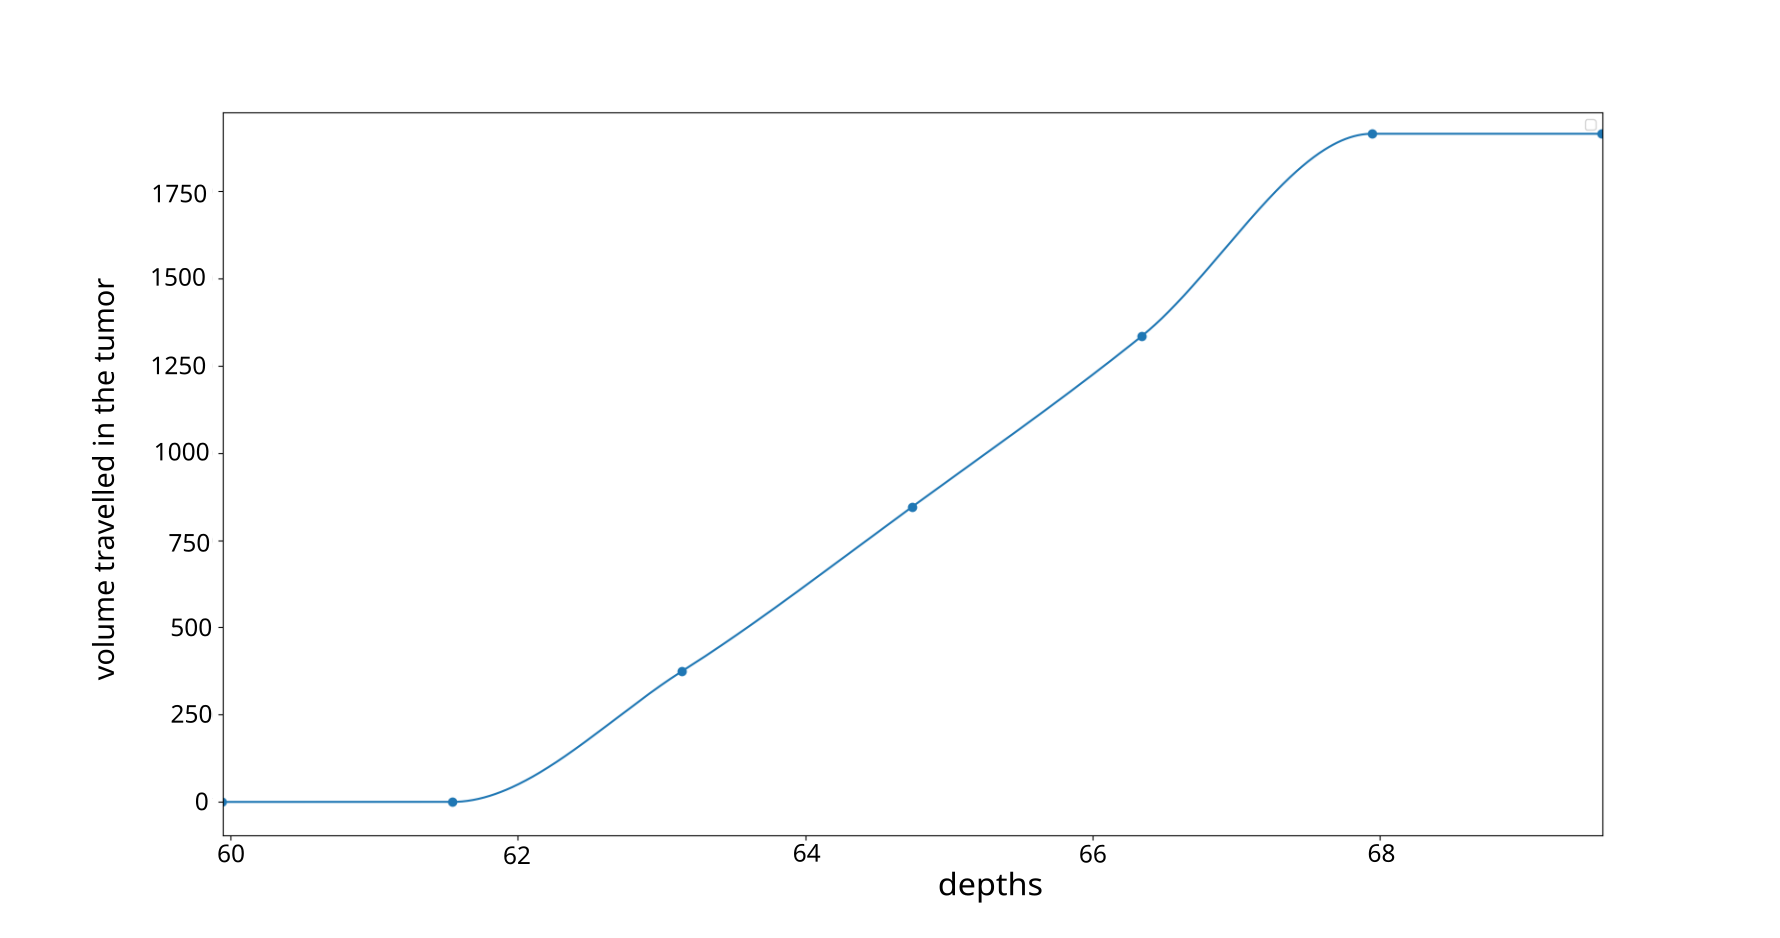
\includegraphics[scale = 0.25]{./images/plot_depth_volume_2.png}
    \caption{graphique de la distribution cumulée du volume (en $mm^3$) de la tumeur du troisième patient CCK selon la profondeur (en $mm$) pour une tumeur donnée. Les points correspondent aux slices enregistrées dans l'image sitk (avec son spacing initial). La courbe est obtenue par interpolation de ces points via des splines cubiques de Hermite.}
    \label{fig:depth_volume}
\end{figure}

\subsubsection{Extraction de partie de foie saine}
Nous avons voulu rajouter les features obtenue en réalisant l'extraction sur des portions de foie sain. En effet, les radiologues comparent généralement la luminosité de la zone tumorale au reste du foie et il nous semblait donc pertinent de faire de même avec notre modèle.\\
\indent Pour ce faire, on a extrait autour de la zone tumorale un petit liseret de tissus. Afin d'être cetain de ne pas englober de zone hors du foie ou traversée par un vaisseau sanguin, nous avons décidé de n'extraire que des zones de faible variance locale et dont la luminosité est plus grande que celle de l'arrière plan noir. En ajoutant un critère de connexité 3D, on peut extraire une zone 3D de foie sain assez conséquente pour y réaliser une extraction 3D des features de firstorder et de texture (la forme de la zone extraite n'ayant pas d'intérêt).\\
\indent Afin d'être certain d'extraire la même zone de tissu sain dans les différentes radios d'une même tumeur, on a décidé de ne détourer le tissu sain que sur la radio tardive (c'était à ce temps que, visuellement, notre méthode d'extraction réussissait le mieux). Puis on a appliqué le même détourage sur les autres radios, en décalant légèrement la zone extraite pour tenir compte des mouvements du patient. Ces mouvements étaient estimés en comparant les aires tumorales sur chaque slice et en essayant d'augmenter autant que possible l'intercorrélation des courbes d'aire entre chaque radio et la radio tardive. Cette procédure est effectuée selon les trois axes de l'espace. Finalement, on peut visualiser la zone extraite, comme en Fig. \ref{fig:healthy_zone} afin de contrôler que l'extraction se passe correctement.\\
\indent Cependant, nous n'avons pas perçu d'amélioration dans les performances de nos modèles en rajoutant ces features. Nous avons donc décidé de ne pas les inclure dans la suite de notre étude.\\

\begin{figure}[tbp]
    \centering
    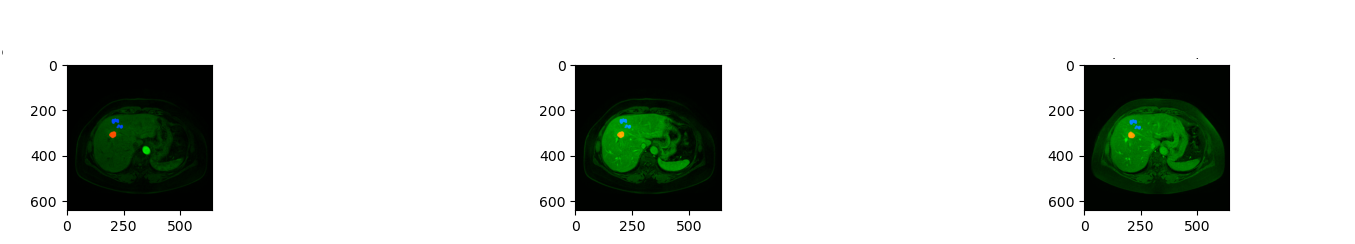
\includegraphics[scale = 0.3]{./images/sain.png}
    \caption{Radios d'une slice d'une tumeur CCK avec en rouge la zone tumorale et en bleu la zone périphérique de foie sain extraite. De gauche à droite on a la radio au temps artériel, la radio au temps portal et la radio au temps tardif. Les axes sont gradués en mm}
    \label{fig:healthy_zone}
\end{figure}


\subsection{Simulated data}


\vspace{10 pt}













\vspace{2 cm}

\section{results}




\section*{Conclusions}
\blindtext




\bibliographystyle{ieeetr} %alpha, apalike, ieeetr
\bibliography{bibliography.bib}

\newpage

\appendix

\section{Annexe A: Paramètres utilisés pour l'extraction de features par pyradiomics}
\label{annexeA}

Liste des paramètres utilisés pour l'extraction de features par pyradiomics:

\subsection{Pour l'extraction 3D de la tumeur}
 
\begin{itemize}[label = $\bullet$]
    \item Bin width : 25
    \item Resampled Pixel Spacing : $[2,2,2]$
    \item interpolator : sitkBSpline
    \item force2D : True
    \item force2Ddimension : 2
\end{itemize}





\end{document}